\documentclass{article}

\usepackage{fancyhdr}
\usepackage{extramarks}
\usepackage{amsmath}
\usepackage{amsthm}
\usepackage{amsfonts}
\usepackage{tikz}
\usepackage[plain]{algorithm}
\usepackage{algpseudocode}
\usepackage{tikz,pgfplots,multicol}

\usetikzlibrary{automata,positioning}

%
% Basic Document Settings
%

\topmargin=-0.45in
\evensidemargin=0in
\oddsidemargin=0in
\textwidth=6.5in
\textheight=9.0in
\headsep=0.25in

\linespread{1.1}

\pagestyle{fancy}
\lhead{\hmwkAuthorName}
\chead{\hmwkClass\ (\hmwkClassInstructor\ \hmwkClassTime)}
\rhead{\hmwkTitle}
\lfoot{\lastxmark}
\cfoot{\thepage}

\renewcommand\headrulewidth{0.4pt}
\renewcommand\footrulewidth{0.4pt}

\setlength\parindent{0pt}

\setcounter{secnumdepth}{0}
\newcounter{partCounter}
\newcounter{homeworkProblemCounter}
\setcounter{homeworkProblemCounter}{1}
\nobreak\extramarks{Problem \arabic{homeworkProblemCounter}}{}\nobreak{}

%
% Homework Problem Environment
%
% This environment takes an optional argument. When given, it will adjust the
% problem counter. This is useful for when the problems given for your
% assignment aren't sequential. See the last 3 problems of this template for an
% example.
%
\newenvironment{homeworkProblem}[1][-1]{
    \ifnum#1>0
        \setcounter{homeworkProblemCounter}{#1}
    \fi
    \section{Problem \arabic{homeworkProblemCounter}}
    \setcounter{partCounter}{1}
    \enterProblemHeader{homeworkProblemCounter}
}{
    \exitProblemHeader{homeworkProblemCounter}
}

%
% Homework Details
%   - Title
%   - Due date
%   - Class
%   - Section/Time
%   - Instructor
%   - Author
%

\newcommand{\hmwkTitle}{HW \#1}
\newcommand{\hmwkDueDate}{January 19, 2017}
\newcommand{\hmwkClass}{MATH 1300}
\newcommand{\hmwkClassTime}{Section 005}
\newcommand{\hmwkClassInstructor}{Professor Braden Balentine}
\newcommand{\hmwkAuthorName}{\textbf{John Keller}}

%
% Title Page
%

\title{
    \vspace{2in}
    \textmd{\textbf{\hmwkClass:\ \hmwkTitle}}\\
    \normalsize\vspace{0.1in}\small{Due\ on\ \hmwkDueDate\ at 10:00am}\\
    \vspace{0.1in}\large{\textit{\hmwkClassInstructor\ \hmwkClassTime}}
    \vspace{3in}
}

\author{\hmwkAuthorName}
\date{}

\renewcommand{\part}[1]{\textbf{\large Part \Alph{partCounter}}\stepcounter{partCounter}\\}

%
% Various Helper Commands
%

% Useful for algorithms
\newcommand{\alg}[1]{\textsc{\bfseries \footnotesize #1}}

% For derivatives
\newcommand{\deriv}[1]{\frac{\mathrm{d}}{\mathrm{d}x} (#1)}

% For partial derivatives
\newcommand{\pderiv}[2]{\frac{\partial}{\partial #1} (#2)}

% Integral dx
\newcommand{\dx}{\mathrm{d}x}

% Alias for the Solution section header
\newcommand{\solution}{\textbf{\large Solution}}

% Probability commands: Expectation, Variance, Covariance, Bias
\newcommand{\E}{\mathrm{E}}
\newcommand{\Var}{\mathrm{Var}}
\newcommand{\Cov}{\mathrm{Cov}}
\newcommand{\Bias}{\mathrm{Bias}}

\begin{document}

\maketitle

\pagebreak


\section{Section 1.1}

\begin{enumerate}
\setcounter{enumi}{11}
	\item Three runners compete in a 100-meter race. The graph depicts the distance run as a function of time for each runner. Describe in words what the graph tells you about this race. Who won the race? Did each runner finish the race? \newline\begin{center}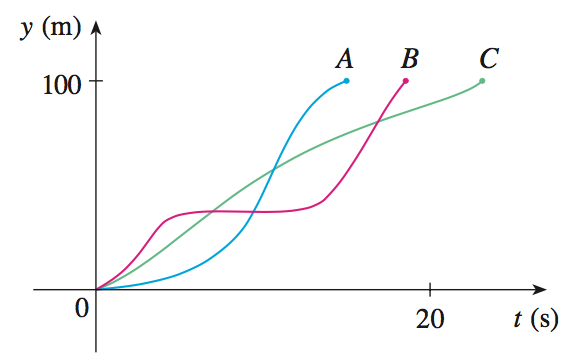
\includegraphics[width=140px]{images/hw1pr12}\newline\end{center}
	The winner of the race is runner A, with runners B and C following closely behind. All three runners did finish the race, which can be determined by all three runners stopping at the same maximum distance (100m).

\setcounter{enumi}{51}
  \item Find an expression for the function whose graph is the given curve: \newline
  \begin{center}
  \pgfplotsset{compat=1.6,width=5cm,height=4cm, every tick label/.append style={font=\small}}
  \pgfplotsset{soldot/.style={color=blue,only marks,mark=*}} \pgfplotsset{holdot/.style={color=blue,fill=white,only marks,mark=*}}
 			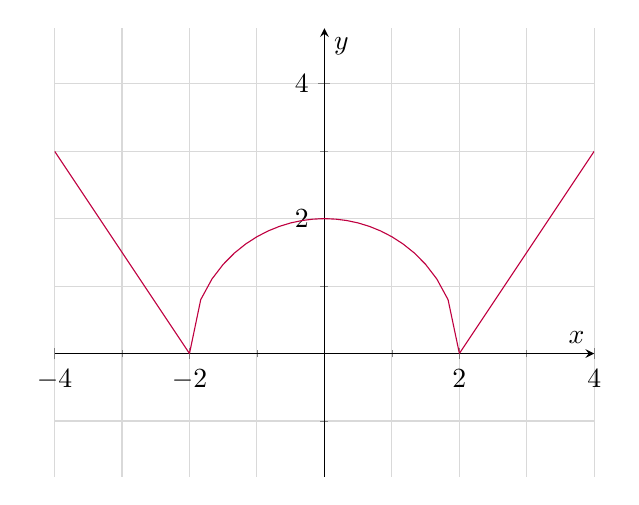
\begin{tikzpicture}
				\begin{axis}[axis lines=middle,xlabel=$x$,ylabel=$y$,axis equal,grid=both,minor tick num=1,grid style={solid, gray!30}]
					\addplot[domain=-4:-2,purple] {-1.5*x-3};
					\addplot[domain=-2:2,purple] {sqrt(2^2-x^2)};
					\addplot[domain=2:4,purple] {1.5*x-3};
				\end{axis}
			\end{tikzpicture} 
  \end{center}
  $$f(x)=\begin{cases} 
      		-\frac{3}{2}x-3, & -4 \leq x < -2 \\
      		\sqrt{2^2-x^2}, & -2 \leq x \leq 2 \\
      		\frac{3}{2}x-3, & 2 < x \leq 4.
   		\end{cases}$$
	
\setcounter{enumi}{59}
  \item An electricity company charges its customers a base rate of \$10 a month, plus 6 cents per kilowatt-hour (kWh) for the first 1200 kWh and 7 cents per kWh for all usage over 1200 kWh. Express the monthly cost $E$ as a function of the amount $x$ of electricity used. Then graph the function $E$ for $0\leq x \leq 2000$.
  		\newline
  		$$E(x)=\begin{cases} 
      		10+0.6x, & 0\leq x\leq 1200 \\
      		10+0.6\times 1200 + 0.07(x-1200), & x > 1200.
   		\end{cases}$$
 		\newline 
 		\begin{center}
 		\pgfplotsset{compat=1.6,width=0.5\linewidth,height=6cm}
		\pgfplotsset{soldot/.style={color=blue,only marks,mark=*}} \pgfplotsset{holdot/.style={color=blue,fill=white,only marks,mark=*}}
 			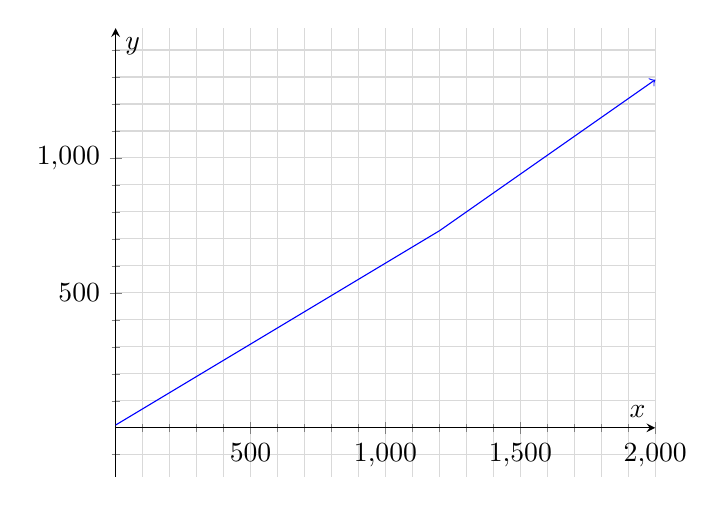
\begin{tikzpicture}
				\begin{axis}[axis lines=middle,xlabel=$x$,ylabel=$y$,axis equal,grid=both,minor tick num=4,grid style={solid, gray!30}]
					\addplot[domain=0:1200,blue] {10+0.6*x};
					\addplot[->,domain=1200:2000,blue] {10+0.6*1200+0.7*(x-1200)};
				\end{axis}
			\end{tikzpicture}
		\end{center}
   		
\setcounter{enumi}{65}
  \item A function $f$ has domain [-5,5] and a portion of its graph is shown. \newline\begin{center}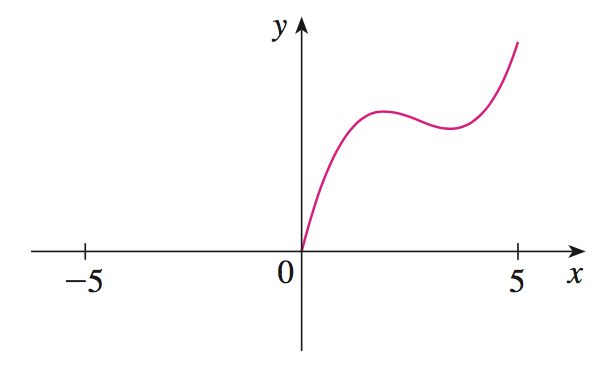
\includegraphics[width=140px]{images/hw1pr66}\end{center}
 \begin{enumerate}
 	\item Complete the graph of $f$ if it is known that $f$ is even.
		\newline \begin{center}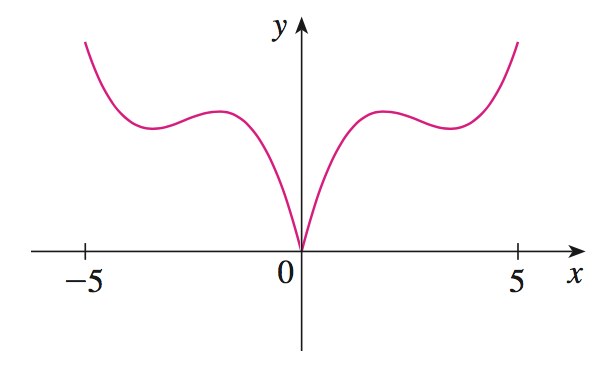
\includegraphics[width=140px]{images/hw1pr66a}\end{center}
 	\item Complete the graph of $f$ if it is known that $f$ is odd.
 		\newline\begin{center}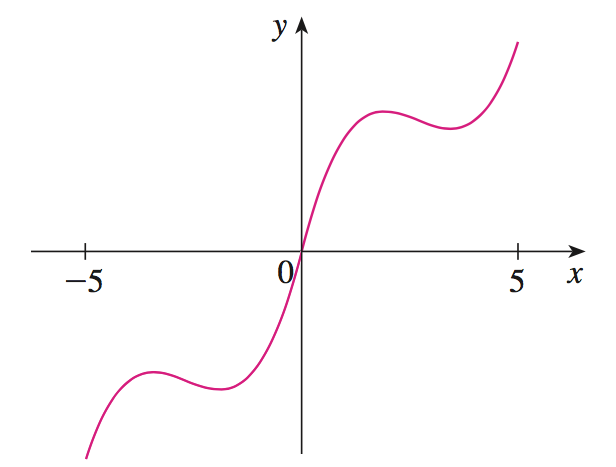
\includegraphics[width=140px]{images/hw1pr66b}\end{center}
 \end{enumerate}
\setcounter{enumi}{73}
 \item If $f$ and $g$ are both even functions, is the product $fg$ even? If $f$ and $g$ are both odd functions, is $fg$ odd? What if $f$ is even and $g$ is odd? Justify your answers.

\begin{figure}[!htb]
\minipage{0.32\textwidth}
  \begin{table}[H]
    \begin{tabular}{cc|cc|cc}
    \multicolumn{2}{c}{$f(x)$} & \multicolumn{2}{c}{$g(x)$} & \multicolumn{2}{c}{$f\cdot g$} \\
    \multicolumn{2}{c}{(even)} & \multicolumn{2}{c}{(even)} & \multicolumn{2}{c}{(even)} \\ \hline
        -2 & 3 & -2 & 10 & -2 & 30 \\ 
        -1 & 1 & -1 & 5 & -1 & 5 \\ 
        0 & 0 & 0 & 0 & 0 & 0 \\
        1 & 1 & 1 & 5 & 1 & 5 \\ 
        2 & 3 & 2 & 10 & 2 & 30 \\ 
    \end{tabular}
\end{table}
\endminipage\hfill
\minipage{0.32\textwidth}
  \begin{table}[H]
    \begin{tabular}{cc|cc|cc}
    \multicolumn{2}{c}{$f(x)$} & \multicolumn{2}{c}{$g(x)$} & \multicolumn{2}{c}{$f\cdot g$} \\
    \multicolumn{2}{c}{(even)} & \multicolumn{2}{c}{(odd)} & \multicolumn{2}{c}{(odd)} \\ \hline
        -2 & 3 & -2 & -10 & -2 & -30 \\ 
        -1 & 1 & -1 & -5 & -1 & -5 \\ 
        0 & 0 & 0 & 0 & 0 & 0 \\
        1 & 1 & 1 & 5 & 1 & 5 \\ 
        2 & 3 & 2 & 10 & 2 & 30 \\ 
    \end{tabular}
\end{table}
\endminipage\hfill
\minipage{0.32\textwidth}%
\begin{table}[H]
    \begin{tabular}{cc|cc|cc}
    \multicolumn{2}{c}{$f(x)$} & \multicolumn{2}{c}{$g(x)$} & \multicolumn{2}{c}{$f\cdot g$} \\
    \multicolumn{2}{c}{(odd)} & \multicolumn{2}{c}{(odd)} & \multicolumn{2}{c}{(even)} \\ \hline
        -2 & -3 & -2 & -10 & -2 & 30 \\ 
        -1 & -1 & -1 & -5 & -1 & 5 \\ 
        0 & 0 & 0 & 0 & 0 & 0 \\
        1 & 1 & 1 & 5 & 1 & 5 \\ 
        2 & 3 & 2 & 10 & 2 & 30 \\ 
    \end{tabular}
\end{table}
\endminipage
\end{figure}

As demonstrated by the three tables above, when $f(x)$ and $g(x)$ are both even, $f\cdot g$ is even. When $f(x)$ is even and $g(x)$ is odd, $f\cdot g$ is odd. When $f(x)$ and $g(x)$ are both odd, $f\cdot g$ is even.

\end{enumerate}


\section{Section 1.2}
\begin{enumerate}
\setcounter{enumi}{17}
	\item The monthly cost of driving a car depends on the number of miles driven. Lynn found that in May it cost her \$380 to drive 480 mi and in June it cost her \$460 to drive 800 mi.
	\begin{enumerate}
		\item Express the monthly cost $C$ as a function of the distance driven $d$, assuming that a linear relationship gives a suitable model.
		\newline 
		\begin{itemize}
			\item Calculating the slope: $$\frac{460-380}{800-480}=\frac{80}{320}=\frac{1}{4}$$
			\item Point-slope formula: $$C-380=\frac{1}{4}(d-180)=\frac{d}{4}-120$$
			\item Simplifying: $$C(d)=\frac{d}{4}+260$$
		\end{itemize}
		\item Use part (a) to predict the cost of driving 1500 miles per month.
		$$C(1500)=\frac{1500}{4}+260=375+260=635$$
		\item Draw the graph of the linear function. What does the slope represent?
		\begin{center}
			\pgfplotsset{compat=1.6,width=0.6\linewidth,height=7cm}
			\pgfplotsset{soldot/.style={color=blue,only marks,mark=*}}\pgfplotsset{holdot/.style={color=blue,fill=white,only marks,mark=*}}
 			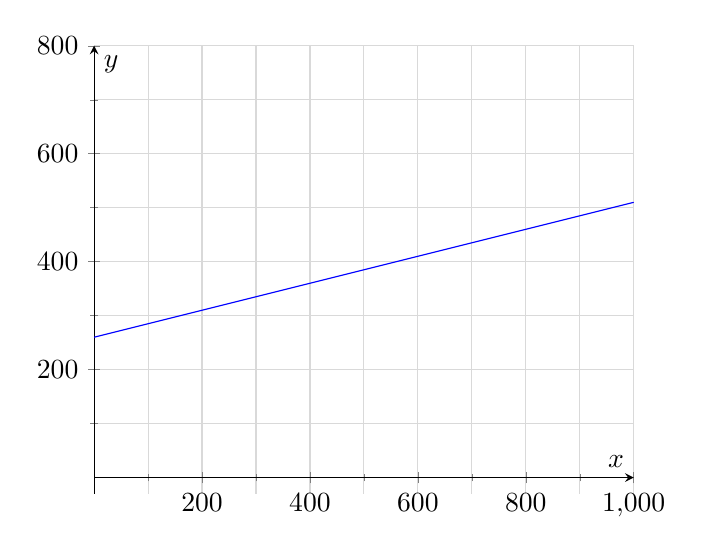
\begin{tikzpicture}
				\begin{axis}[axis lines=middle,xlabel=$x$,ylabel=$y$,axis equal,grid=both,minor tick num=1,grid style={solid, gray!30}]
					\addplot[domain=0:1000,blue] {(x/4)+260};
				\end{axis}
			\end{tikzpicture}
		\end{center}
		The slope reflects the cost per mile driven.
		\item What does the $C$-intercept represent?\newline
		The $C$-intercept represents the starting value, which in this case is how much it costs to own a car (\$260).
		\item Why does a linear function give a suitable model in this situation?\newline
		This is a suitable model because it is expected that the cost per mile driven is proportional across a car's lifespan.
	\end{enumerate}
\end{enumerate}

\section{Section 1.3}

\begin{enumerate}
\setcounter{enumi}{3}
	\item The graph of $f$ is given. Draw the graphs of the following functions.
	\begin{center}
 		\pgfplotsset{compat=1.6,width=5cm,height=5cm}
		\pgfplotsset{soldot/.style={color=blue,only marks,mark=*}} \pgfplotsset{holdot/.style={color=blue,fill=white,only marks,mark=*}}
 			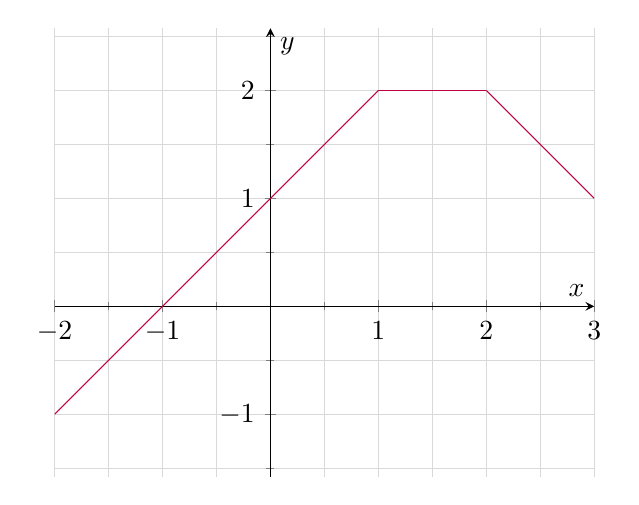
\begin{tikzpicture}
				\begin{axis}[axis lines=middle,xlabel=$x$,ylabel=$y$,axis equal,grid=both,minor tick num=1,grid style={solid, gray!30}]
					\addplot[domain=-2:1,purple] {x+1};
					\addplot[domain=1:2,purple] {2};
					\addplot[domain=2:3,purple] {-x+4};
				\end{axis}
			\end{tikzpicture}
		\end{center}
	\begin{multicols}{2}
	\begin{enumerate}
		\item $y=f(x)-2$ \\
		\pgfplotsset{compat=1.6,width=5cm,height=5cm}
		\pgfplotsset{soldot/.style={color=blue,only marks,mark=*}} \pgfplotsset{holdot/.style={color=blue,fill=white,only marks,mark=*}}
 			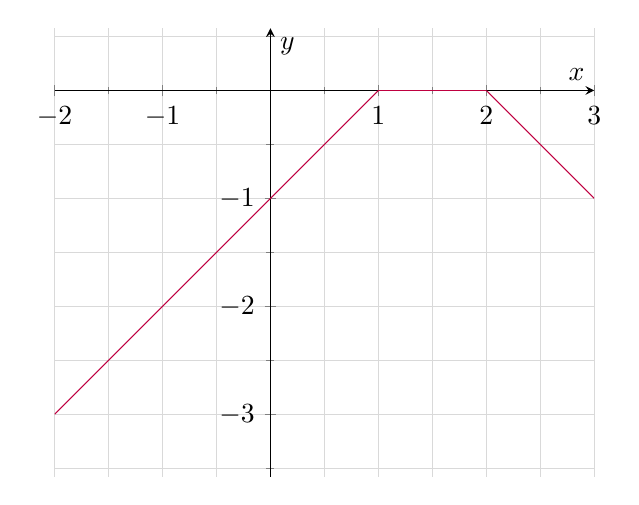
\begin{tikzpicture}
				\begin{axis}[axis lines=middle,xlabel=$x$,ylabel=$y$,axis equal,grid=both,minor tick num=1,grid style={solid, gray!30}]
					\addplot[domain=-2:1,purple] {(x+1)-2};
					\addplot[domain=1:2,purple] {2-2};
					\addplot[domain=2:3,purple] {-x+4-2};
				\end{axis}
			\end{tikzpicture}
		\item $y=f(x-2)$ \\
		\pgfplotsset{compat=1.6,width=5cm,height=5cm}
		\pgfplotsset{soldot/.style={color=blue,only marks,mark=*}} \pgfplotsset{holdot/.style={color=blue,fill=white,only marks,mark=*}}
 			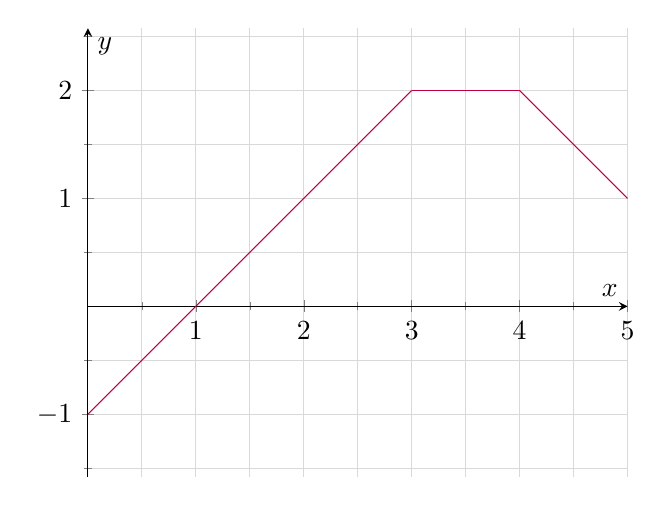
\begin{tikzpicture}
				\begin{axis}[axis lines=middle,xlabel=$x$,ylabel=$y$,axis equal,grid=both,minor tick num=1,grid style={solid, gray!30}]
					\addplot[domain=0:3,purple] {(x-2)+3-2};
					\addplot[domain=3:4,purple] {2};
					\addplot[domain=4:5,purple] {-(x)+3+2+1};
				\end{axis}
			\end{tikzpicture}
		\item $y=-2f(-x)$ \\
		\pgfplotsset{compat=1.6,width=5cm,height=5cm}
		\pgfplotsset{soldot/.style={color=blue,only marks,mark=*}} \pgfplotsset{holdot/.style={color=blue,fill=white,only marks,mark=*}}
 			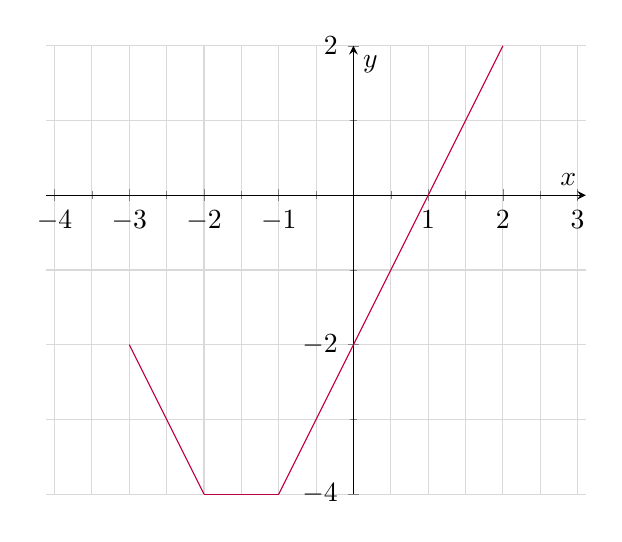
\begin{tikzpicture}
				\begin{axis}[axis lines=middle,xlabel=$x$,ylabel=$y$,axis equal,grid=both,minor tick num=1,grid style={solid, gray!30}]
					\addplot[domain=-1:2,purple] {2*(x)-6+4};
					\addplot[domain=-2:-1,purple] {-4};
					\addplot[domain=-2:-3,purple] {2*(-x)-6-2};
				\end{axis}
			\end{tikzpicture}
		\item $y=f(\frac{1}{3}x)+1$ \\
		\pgfplotsset{compat=1.6,width=5cm,height=5cm}
		\pgfplotsset{soldot/.style={color=blue,only marks,mark=*}} \pgfplotsset{holdot/.style={color=blue,fill=white,only marks,mark=*}}
 			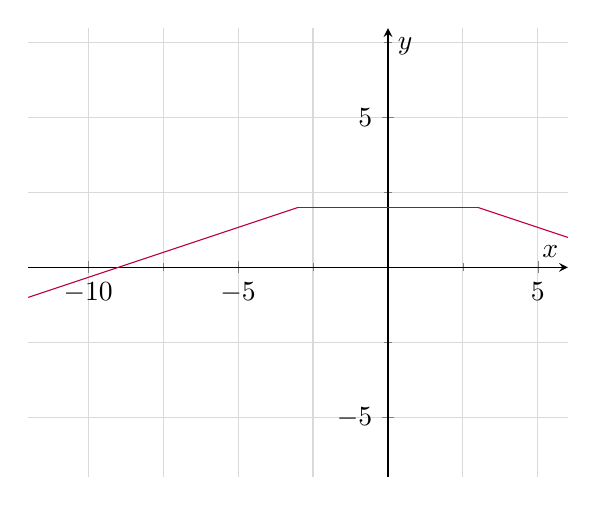
\begin{tikzpicture}
				\begin{axis}[axis lines=middle,xlabel=$x$,ylabel=$y$,axis equal,grid=both,minor tick num=1,grid style={solid, gray!30}]
					\addplot[domain=-12:-3,purple] {((1/3)*x)+3};
					\addplot[domain=-3:3,purple] {2};
					\addplot[domain=3:6,purple] {-(1/3)*x+3};
				\end{axis}
			\end{tikzpicture}
	\end{enumerate}
	\end{multicols}
\setcounter{enumi}{53}
\item A spherical balloon is being inflated and the radius of the balloon is increasing at a rate of 2 cm/s.
	\begin{enumerate}
		\item Express the radius $r$ of the balloon as a function of the time $t$ in seconds.
		\newline $$r(t)=t2$$
		\item If $V$ is the volume of the balloon as a function of the radius, find $V \circ r$ and interpret it.
		\newline $$(V \circ r)(t)=\frac{4}{3}\pi (2t)^3$$
		\newline This equation represents how the volume of the balloon changes over time. This was obtained by using the equation for volume of a sphere ($\frac{4}{3}\pi r^3$) and inserting the equation from (A) for $r$.
	\end{enumerate}
\setcounter{enumi}{59}
\item If you invest $x$ dollars at 4\% interest compounded annually, then the amount $A(x)$ of the investment after one year is $A(x)=1.04x$. Find $A\circ A$, $A  \circ A  \circ A$, and $A \circ  A \circ  A \circ  A$. What do these compositions represent? Find a formula for the composition of $n$ copies of $A$.
	\begin{enumerate}
		\item $A\circ A$ = $1.04\cdot 1.04 = 1.0816$
		\item $A  \circ A  \circ A$ = $1.04\cdot 1.04\cdot 1.04 = 1.124864$
		\item $A \circ  A \circ  A \circ  A$ = $1.04\cdot 1.04\cdot 1.04\cdot 1.04 = 1.16985856$
	\end{enumerate}
	The above three operations represent compounding of interest over time.
	$$A(n)=1.04^n$$
\setcounter{enumi}{61}
\item If $f(x)=x+4$ and $h(x)=4x-1$, find a function $g$ such that $g \circ f=h$.
\newline $$g(x)=4x-17$$
\end{enumerate}

\section{Challenge Question}
Find a formula for a function $f(x)$ such that:
\begin{itemize}
\item $f(3)=0$
\item $f(x)$ is even
\item $f$ has a horizontal asymptote at $y=2$
\item $f$ has a vertical asymptotes at $x=4$ and $x=-4$
\item $f(0)=1$ (Meeting this requirement is the trickiest part!) 
\end{itemize}

$$f(x)=\frac{x^2-2}{x^2-16}+1$$
\begin{center}
The above equation meets all requirements except for the last one, $f(0)=1$.

$$f(x)=\frac{x^2}{x^2-16}+1$$
This equation meets all requirements except for the first one, $f(3)=0$.

$$f(x)=\begin{cases} 
      		\frac{x^2-2}{x^2-16}+1, & x < 0 \\
      		1, & x = 0 \\
      		\frac{x^2-2}{x^2-16}+1, & x > 0.
   		\end{cases}$$
This equation meets all requirements, no exceptions.

\end{center}



\end{document}
